% 2008 年江苏卷第 15 题：单位圆上两点 A、B，终边与 Ox 轴成锐角 α、β。
% 来源 PDF：gaokaomath-src/普通高考/2008/2008江苏.pdf
% SHA-256：b998b93963143559a1ce800a6d320de618883b0e22ee5130b7666a2374caeba0
% 原页：2008江苏.pdf 第 1 页（A3 三栏）第 2 栏，书页码 457。
% 绘制依据：按原页画单位圆、x/y 轴、O，A 在第一象限靠近 y 轴、B 在第一象限靠近 x 轴，
%   α、β 分别标在 OA、OB 与 x 轴之间。
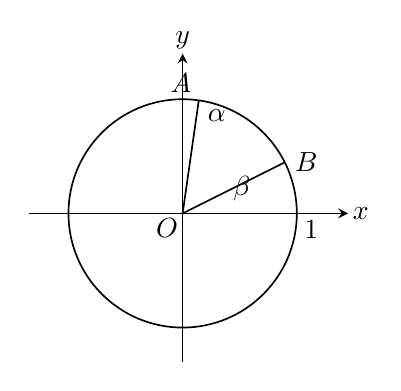
\begin{tikzpicture}[scale=1.45, semithick, every node/.style={inner sep=1.4pt}]
  \draw (0,0) circle [radius=1];
  \draw[->,>=stealth] (-1.35,0) -- (1.45,0) node[right] {$x$};
  \draw[->,>=stealth] (0,-1.3) -- (0,1.4) node[above] {$y$};
  \node[below left] at (0,0) {$O$};

  \coordinate (A) at (0.1414,0.9899);
  \coordinate (B) at (0.8944,0.4472);

  \draw (0,0) -- (A);
  \draw (0,0) -- (B);

  \node[above left=1pt] at (A) {$A$};
  \node[right=2pt] at (B) {$B$};
  \node at (0.30,0.86) {$\alpha$};
  \node at (0.52,0.22) {$\beta$};
  \node[below right=1pt] at (1,0) {$1$};
\end{tikzpicture}
